\section{Introduction}

BGP (Border Gateway Protocol) is the critical infrastructure for the Internet
and interdomain routing. The routing protocol operates at the junction point
where independent networks (ASes, or autonomous systems) exchange network
traffic through proscribed and announced routes of connectivity. Because ASes
are separate networking and economic entities, BGP must operate, while
balancing essentially two purposes, which are not entirely orthogonal to one
another: the limits of delivering efficiently routed network traffic and the
realities of routing policies, which are governed by operating costs, a number
of policy-based and politically-based issues, network locality, multihoming
preferences and, in some select cases, traffic connection capacity. These have
functioned, mostly together and at times as trade-offs to one another, to
increase complexity within BGP and to deliver the present level of routed
Internet traffic -- together with its policy-bound routing inefficiencies --
as is seen at this time.

As originally envisioned, a hierarchical and scalable routing table was to
serve as an efficient and streamlined mechanism. However, not foreseen was the
degree to which the limited number of IPv4 addresses ($2^{32}$) and the
increasing number of allocations to users would lead to fractionalization and
finer segmentation of the IP address space. Fragmentation has effectively
flattened portions of the IP address table, rather than preserved the
hierarchical IP address-based routing. Reasons for numerous "special-case"
announcements include multihoming demands and Internet customers'
implementation of particular traffic engineering to suit any special purposes.
Likewise, individual institutions have grown to need more IP addresses than
originally allocated and received additional address blocks that are
non-adjacent. In either case, the routing table has expanded enormously over
the past ten years, with the table maintaining more entries than a
hierarchical structure would have yielded that worked with strictly
consolidated blocks. Figure~\ref{fig:BGP vs RIR}, for example, that over the
time interval of this current study (2003-2009), the number of table entries
increased from a little of double number of allocated IP blocks to over three
times the number of blocks. To account for this, correspondingly, the Internet
has handled an increasing number of transmitted BGP updates to propagate these
steadily ongoing changes.

\begin{figure}[htbp]
	\centering
		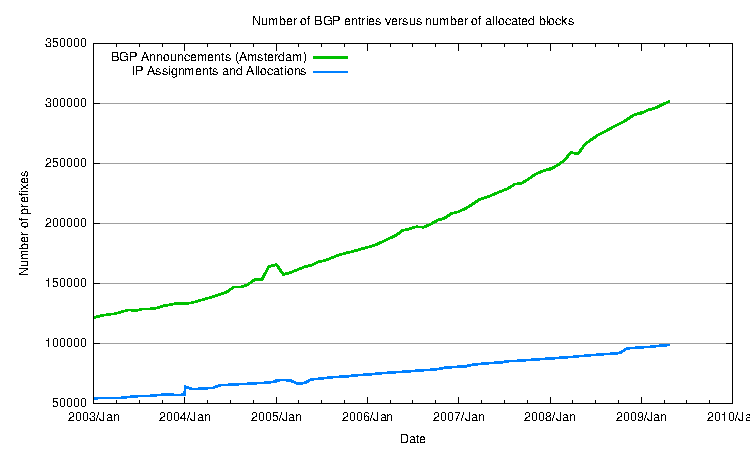
\includegraphics[width=\columnwidth]{01_bgp_ip_size/02_bgp_max_vs_ip}
	\caption{Number of BGP entries compared to number of allocated IP blocks}
	\label{fig:BGP vs RIR}
\end{figure}

There is an interesting aspect to notice with the BGP table growth. While the
routing table has undergone a substantial growth (compared to the number of
new allocated IP spaces), all the IP space that these announcements cover is
still only a fraction of the total measured IP space that has been allocated.
This is illustrated in Figure~\ref{fig:BGP vs RIR space}, which illustrates
that over time, the amount of dormant IP space -- allocated, but not
announced in routing tables -- has ranged from a little over 1/3 to a little
over 1/4 of the total as unused. Despite many fragmented announcements in the
BGP table, the amount of IP space still unused has not dipped below the 25\%
mark yet, of what is available at a given time.

\begin{figure}[htbp]
	\centering
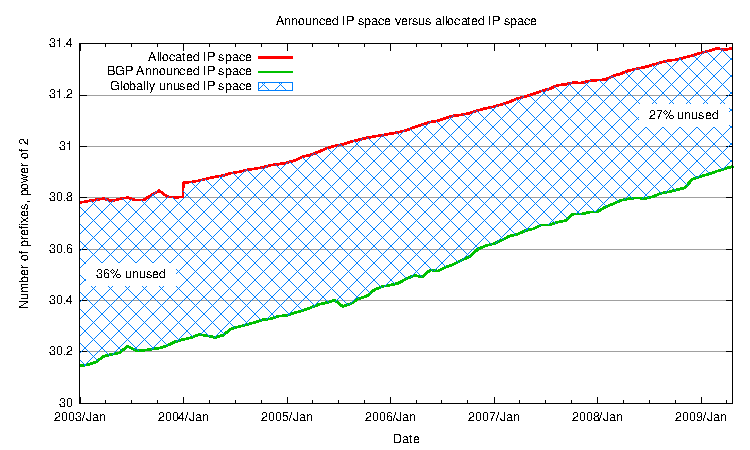
\includegraphics[width=\columnwidth]{01_bgp_ip_size/02_bgp_max_vs_ip_space}
	\caption{Comparing the IP space that has been allocated to the amount of IP space announced in the BGP table}
	\label{fig:BGP vs RIR space}
\end{figure}

In this paper we update and expand on some of the done previously by Meng et
al. \cite{Meng:2005:IPv4-address}. The prior research reported a number of
statistics that serve as a baseline for our project. These include 1) the
number of allocated blocks and 2) the number of announced prefixes. First, we
analyze dynamics of IP address allocation. We share the recent history of
which prefix block sizes are most popular to allocate to ISPs (Internet
Service Providers). We show when IP prefixes have been allocated, as viewed on
a yearly basis, and link this activity to regions of the world where such
allocations have been requested. We then summarize where the most changes have
occurred, which indicate where the busiest Internet areas around the world are
and, more importantly, identify as well the regions globally where there has
been the most rapid development of ISP hosting. Second, we turn from IP prefix
allocation and and examine the correlation to the contents of the BGP routing
table. From the common prefix block sizes to allocate, we share what sized
blocks are more typical to be included in the BGP table. On a related note, we
examine the age, or lifespan, of BGP entries as measured between 2003 and
2009. We present, as before with IP address block allocations, a summary by
geography of which regions of the globe contribute to the BGP table contents
each year. It will be possible to draw some conclusions about a country's
"efficiency" of its IP prefix announcement: a measure of how much IP space
allocated to a country is effectively routed with the fewest announcements in
the BGP routing table. We also discuss a number of factors that contribute to
the marked growth in the routing table.

The paper is organized as follows. Section~\ref{sec:data sets} describes the
data sets and methodology used in our study. Section~\ref{sec:allocations} presents statistics for
IP address allocation and several of the dynamics happening regionally. In
Section~\ref{sec:bgp} we analyze the composition of the BGP table and its changes over
time, as well as the longevity and stability of routing table entries.
Finally, we present related work and conclusions in Sections~\ref{sec:related_work} and \ref{sec:conclusions}.

% The existing Internet fully relies on the BGP protocol~\cite{Rekhter:1995:RFC1771-BGP} to maintain global connectivity. The key element of the BGP is that each participant (autonomous system, AS) announces its IP prefixes which are propagated to the rest of the ASes by means of the protocol. Although the announced set is generally limited by the address blocks allocated to a particular AS by a Regional Internet Registry (RIR), the AS itself decides the granularity of the announcements. In other words, ASes having only one allocated address block can announce multiple prefixes. The two major reasons for this are traffic engineering and multihoming. The popularity of this prefix splitting can be demonstrated by allocation vs announcement statistics. The number of announced prefixes (160K in 2004~\cite{Meng:2005:IPv4-address} growing 300K in 2009~\cite{::BGP-Reports}) is more than two times the number of allocated IPv4 blocks (65K in 2004, 140K in 2009 respectively). These dynamics cast doubt on global routing scalability.
%
% As originally envisioned, a hierarchical and scalable routing table was to serve as an efficient and streamlined mechanism. However, not foreseen was how the limited number ($2^{32}$) of IPv4 addresses and alongside the increasing number of allocations to users would lead to fractionalization and finer segmentation of the IP address table. There exist several solutions which attempt to contain the size of the global routing table.  Accompanying the growth of the IP assignments have been aggregation techniques with the intent to gather a group of prefixes under a more general IP prefix. However, Internet customers with particular traffic engineering and multihoming demands have preferred that these guidelines not be implemented. On the other hand, some customers willing to aggregate are not in a position to do so, due to the inability of RIRs to assign a specific requester a contiguous range of IP addresses. Such is the case, for example, with UCLA which has accumulated eight IPv4 address blocks and is forced to announce eight different prefixes (128.97.0.0/16, 131.179.0.0/16, 149.142.0.0/16, 164.67.0.0/16, 169.232.0.0/16, 192.35.210.0/24, 192.35.225.0/24, 192.154.2.0/24). This granular allocation has been one of the major contributors to the growth of the global routing table. An interesting topic to pursue would be to find the average number of allocated blocks assigned to various ASes.
%
% Meng et al.~\cite{Meng:2005:IPv4-address} reported a number of statistics that will serve as a baseline for our project.  These include 1) the number of allocated blocks and 2) the number of announced prefixes. We propose to conduct more detailed research by country and AS granularity on the ratio and correlation between the number of allocated blocks and the announced prefixes within the BGP routing table. Arguably, any attempt to renumber allocations such that they are less fragmented would reduce both the number of allocations and correspondingly the number of prefixes and size of the BGP table. Our analysis will help to establish an upper bound of the potential BGP routing table reduction if an IPv4 renumbering technique were to be implemented. Additionally, this will justify the necessity of effective IPv6 address assignment and reassignment techniques.

% picture of total # of prefixes
% picture of total # of IP space

% Section~\ref{sec:} provides an introduction to the Border Gateway Protocol.    Section 4 presents statistics for IP address allocation and announcement and the BGP table growth.  Section 5 concerns the trends of fragmentation in the BGP routing table.  Section 6 draws a connection between locality and routing table growth, and it shows in which parts of the globe Internet connectivity has been expanding over the last several years.  Section 7 presents data on the longevity and stability of routing table entries.  Related work is discussed in Section 8, followed by the conclusion in Section 9.   Section 2to enable routing to these IP address blocksthe distribution of IP prefix announcements per region of the worldWe propose to conduct more detailed research by country and AS granularity on the ratio and correlation between the number of allocated blocks and the announced prefixes within the BGP routing table. Arguably, any attempt to renumber allocations such that they are less fragmented would reduce both the number of allocations and correspondingly the number of prefixes and size of the BGP table. Our analysis will help to establish an upper bound of the potential BGP routing table reduction if an IPv4 renumbering technique were to be implemented. Additionally, this will justify the necessity of effective IPv6 address assignment and reassignment techniques. 
